\chapter{Performance models}\label{ch:perf}

A measurement says how fast a kernel runs; a model says how fast it could run, and why it does not. This chapter
collects the simple models the port uses to judge its measurements \citep{williams2009}. Each model needs a few
numbers about the GPU, which the profiler measures (\cref{ch:prof}); until then the datasheet values of
\cref{tab:gpus} stand in.

\section{The roofline}

A kernel performs $F$ floating-point operations and moves $B$ bytes between the device memory and the chip. Its
\emph{arithmetic intensity} is $I = F/B$. With a peak arithmetic rate $\pi$ and a memory bandwidth $\beta$, the rate
it can reach is bounded by
\begin{equation}
  P \le \min(\pi,\ \beta\, I).
  \label{eq:roofline}
\end{equation}
Below the \emph{ridge point} $I^* = \pi/\beta$ the kernel is limited by memory, above it by arithmetic. In REPRO mode
the peak is half the datasheet value, because no multiply and add are fused:
\begin{itemize}
  \item A100 40~GB: $\pi = 9.75$~TFLOP/s (FP32, no FMA), $\beta = 1.56$~TB/s, $I^* = 6.25$ flop/byte;
  \item H100 SXM: $\pi \approx 33.5$~TFLOP/s, $\beta = 3.35$~TB/s, $I^* \approx 10$ flop/byte.
\end{itemize}

\begin{figure}[ht]
\centering
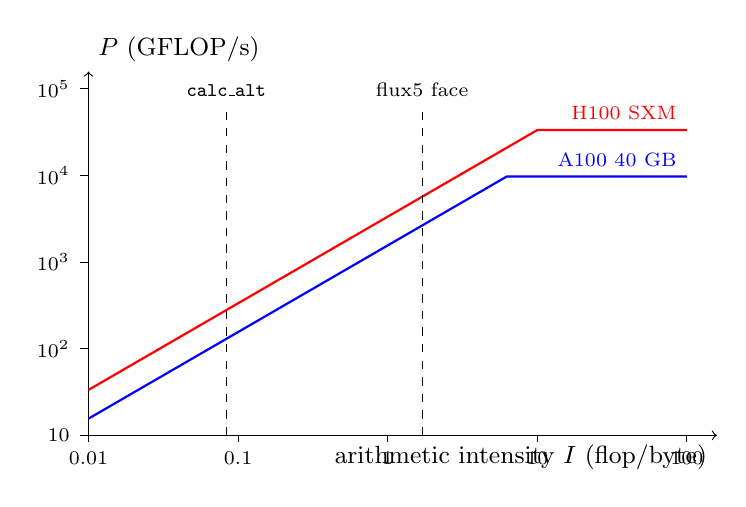
\begin{tikzpicture}[x=1.9cm,y=1.1cm]
  % axes: x = log10(I), y = log10(P in GFLOP/s)
  \draw[->] (-2,1) -- (2.2,1) node[below left, font=\small] {arithmetic intensity $I$ (flop/byte)};
  \draw[->] (-2,1) -- (-2,5.2) node[above right, font=\small] {$P$ (GFLOP/s)};
  \foreach \x/\l in {-2/0.01,-1/0.1,0/1,1/10,2/100} \draw (\x,1) -- (\x,0.92) node[below, font=\scriptsize] {\l};
  \foreach \y/\l in {1/10,2/$10^2$,3/$10^3$,4/$10^4$,5/$10^5$} \draw (-2,\y) -- (-2.06,\y) node[left, font=\scriptsize] {\l};
  % A100 40 GB, REPRO (no FMA)
  \draw[thick, blue] (-2,1.193) -- (0.796,3.989) -- (2,3.989) node[above left, font=\scriptsize] {A100 40 GB};
  % H100 SXM, REPRO (no FMA)
  \draw[thick, red] (-2,1.525) -- (1.0,4.525) -- (2,4.525) node[above left, font=\scriptsize] {H100 SXM};
  % kernels
  \draw[dashed] (-1.079,1) -- (-1.079,4.8) node[above, font=\scriptsize] {\texttt{calc\_alt}};
  \draw[dashed] (0.23,1) -- (0.23,4.8) node[above, font=\scriptsize] {flux5 face};
\end{tikzpicture}
\caption{Roofline of the REPRO build (FP32 without FMA, datasheet ceilings) with the intensities of two kernels
estimated in the text. The measured ceilings and the measured points of the port's kernels are \tbr\ (profiler tasks
PR-H4 and PR-L4.1).}
\label{fig:roofline}
\end{figure}

\paragraph{Two examples.}
\begin{itemize}
  \item \code{calc_alt} (\cref{lst:calc-alt-acc}) adds two values and stores one: one operation for 12 bytes, so
    $I = 1/12 \approx 0.08$. Over the d02 domain ($810 \times 59 \times 810 = 3.9 \times 10^7$ points) it moves
    465~MB and must take at least 298~$\mu$s on an A100 40~GB and 139~$\mu$s on an H100 SXM.
  \item A face flux of 5th-order advection (\cref{ch:adv}) takes about 20 operations: the six-point stencil, the
    upwind correction and the product with the velocity. If the six values of the stencil come from the caches, the
    face costs one value read from memory, one velocity read and one flux written: 12 bytes, $I \approx 1.7$.
\end{itemize}
Both lie far left of either ridge. This is true of almost all of WRF's dynamics: its speed on a GPU is set by the
bytes it moves, not by the operations it performs. Two parts of WRF have higher intensities: column physics, which
does long sequences of operations on a few values per level, and every call of a reproducible elementary function,
which costs some tens of double-precision operations.

\section{The bandwidth floor of a step}

If every kernel moved only the bytes it must (each array it touches read or written once) at the measured bandwidth,
a step would take
\begin{equation}
  T_{\text{floor}} = \sum_{k \in \text{kernels}} \frac{B_k^{\min}}{\beta_{\text{meas}}}.
\end{equation}
The ratio $\eta = T_{\text{floor}}/T_{\text{meas}}$ is the step's efficiency against memory. A kernel with low
$\eta_k$ either moves more than its minimal bytes (uncoalesced access, poor reuse, spills: \cref{ch:memory,ch:tiling})
or does not use the bandwidth at all (too short, too few threads, divergence: \cref{ch:fusion,ch:warp}). The port's
target for memory-bound kernels is 60\,\% of the measured bandwidth (\code{plan.md}, section~11.2). The floor of the
case's step, and the measured efficiency, are \tbr.

\section{Launches and gaps}

Every kernel launch costs time on the host (the runtime prepares the launch) and on the device (the kernel starts and
its blocks are scheduled). When the GPU finishes a kernel before the next one is ready, it idles. A first model of a
step is
\begin{equation}
  T_{\text{step}} \approx \sum_k t_k + n_{\text{launch}}\, t_{\text{gap}},
\end{equation}
where $t_k$ are the kernel times and $t_{\text{gap}}$ the average idle time between kernels, measured by the profiler
(PR-H3, PR-A5). The plan estimates 400 to 500 launches per d02 step.

The model shows why the size of the case matters:
\begin{itemize}
  \item on the full case, one pass over a d02 3D field takes about 100~$\mu$s on an A100 40~GB, so a few
    microseconds of gap per kernel are a few per cent;
  \item on the dev case (d02 $181 \times 60 \times 181$), a field is 7.9~MB and one pass takes about 5~$\mu$s:
    comparable to a launch. The dev case's d02 is launch-bound, and its timings say little about the full case.
\end{itemize}
Fewer launches (fusion), launches that do not wait (asynchronous queues) and launches prepared once and replayed
(CUDA Graphs) reduce the second term (\cref{ch:fusion}).

\section{Transfers}

Data moved between host and device crosses PCIe at tens of GB/s. The model of a phase of the port sums the bytes of
its islands and sync points (task PR-L4.4):
\begin{itemize}
  \item \textbf{Phases 1 to 4.} The bracket of \code{solve_em} downloads and uploads the domain's whole state at every
    call: on the dev case, about 6~GB of d01 state twice per d01 step, about half a second at 25~GB/s. It makes the
    development builds slow, which is acceptable because they are only for testing.
  \item \textbf{Phase 5 onwards.} Only the sync points remain. The largest regular transfer is the nest's ozone field
    after each forcing: 162~MB per d01 step, about 3.3~TB over the 17-hour run, or two to three minutes. Optimization
    O10 uploads it only before the next radiation call of d02.
\end{itemize}
The copies the profiler sees must match the model (T-NSYS); a copy the model does not predict is a bug.

\section{Memory}

The memory model predicts the device memory a case needs, from the Registry and the namelist
(\code{port/gpu_mem_estimate.py}). On two smoke cases it agreed with WRF's own count to within 3.5\,\%. For the
Eaton case it predicts:
\begin{center}
\small
\begin{tabular}{lr}
\toprule
Item & GB \\
\midrule
d01 state ($460 \times 60 \times 460$ memory points) & 6.76 \\
d02 state ($821 \times 60 \times 821$, including the 1.68~GB fire grid) & 24.67 \\
scratch pool & 7.47 \\
work arrays (approximate) & 3.43 \\
RRTMG batch (4096 columns) & 4.51 \\
local memory of column physics & 8.29 \\
context and other & 1.50 \\
\midrule
total & 56.6 \\
\bottomrule
\end{tabular}
\end{center}
This does not fit one of the project's 40~GB A100s. The acceptance case \code{eaton_mid} is sized by the same
estimator to fit one with 15\,\% headroom (gate limit 34~GB), and the full case runs on both GPUs together
(\cref{ch:mgpu}). The measured peaks are \tbr\ (gate G-MEM).

\section{What remains on the host}

Some work stays on the CPU: initialization, the formatting of output, and the interpolation inside the nest forcing.
By Amdahl's law, if a fraction $s$ of the original time stays serial on the host, the speedup cannot exceed $1/s$
however fast the GPU part becomes. The profiler reports the host share of the step as its own range.

\section{Comparing with CPUs}

A GPU speedup is meaningful only against a fair baseline. The port reports three numbers (\cref{ch:results}):
\begin{itemize}
  \item against CPU-REF on the 56 host cores of the same workstation: the same source, compiler and arithmetic,
    on one machine;
  \item against the original CCR run of the case, with its compiler and flags, statistically (that run is not
    reproduced bit for bit, and nothing of the port runs on CCR);
  \item energy to solution: power times time, for the GPUs and for the host cores, for the same simulated hours.
\end{itemize}
And it reports REPRO and FAST side by side once FAST exists. Their difference is the measured cost of
reproducibility (ADR-003).
